\documentclass{article}

% content/resources/templates/preamble.tex
\usepackage[margin=0.6in]{geometry}
\author{Milav Dabgar}
\usepackage{amsmath,amssymb,amsthm}
\usepackage{booktabs}
\usepackage{multirow}
\usepackage{xcolor}
\usepackage{tcolorbox}
\tcbuselibrary{breakable,skins}
\usepackage[colorlinks=true,linkcolor=blue]{hyperref}
\usepackage{titlesec}
\usepackage{enumitem}
\usepackage{tikz}
\usepackage{pgfplots}
\usepackage{circuitikz}
\usepackage[version=4]{mhchem}
\usepackage{longtable}
\usepackage{array}
\usepackage{float}
\usepackage{caption}
\usepackage{listings}

\lstset{
  basicstyle=\small\ttfamily,
  breaklines=true,
  breakatwhitespace=false,
  postbreak=\mbox{\textcolor{red}{$\hookrightarrow$}\space},
  float=false,
  numbers=left,
  numberstyle=\tiny\color{gray},
  numbersep=10pt,
  xleftmargin=2em,
  keywordstyle=\color{blue},
  commentstyle=\color{green!60!black},
  stringstyle=\color{purple},
  backgroundcolor=\color{gray!5},
  showstringspaces=false,
  tabsize=2,
  captionpos=b,
  keepspaces=true,
  columns=flexible
}

\pgfplotsset{compat=1.18}
\usetikzlibrary{shapes,arrows,positioning,calc,patterns,decorations.pathmorphing,decorations.markings,arrows.meta}

% Color scheme
\definecolor{headcolor}{RGB}{0,102,204}
\definecolor{keycolor}{RGB}{220,20,60}
\definecolor{solutioncolor}{RGB}{34,139,34}
\definecolor{mnemoniccolor}{RGB}{148,0,211}
\definecolor{codecolor}{RGB}{0,0,100}

% Spacing
\setlength{\parskip}{3pt}
\setlist[itemize]{nosep}
\setlist[enumerate]{nosep}

% Title formatting
\titleformat{\section}{\Large\bfseries\color{headcolor}}{\thesection}{1em}{}
\titleformat{\subsection}{\large\bfseries\color{headcolor}}{\thesubsection}{1em}{}

% Pandoc tightlist compatibility
\providecommand{\tightlist}{%
  \setlength{\itemsep}{0pt}\setlength{\parskip}{0pt}}

% Pandoc longtable compatibility
\newcounter{none}
\def\thenone{}


% content/resources/templates/english-boxes.tex

% Custom environments
\newtcolorbox{solutionbox}{
 breakable,
 enhanced,
 colback=solutioncolor!5!white,
 colframe=solutioncolor!75!black,
 fonttitle=\bfseries,
 title=Solution
}

\newtcolorbox{solutionboxnobreak}{
 colback=solutioncolor!5!white,
 colframe=solutioncolor!75!black,
 fonttitle=\bfseries,
 title=Solution
}

\newtcolorbox{keyformula}{
 breakable,
 enhanced,
 colback=keycolor!5!white,
 colframe=keycolor!75!black,
 fonttitle=\bfseries,
 title=Key Formula
}

\newtcolorbox{mnemonicboxenv}{
 breakable,
 enhanced,
 colback=mnemoniccolor!5!white,
 colframe=mnemoniccolor!75!black,
 fonttitle=\bfseries,
 title=Mnemonic
}

\newcommand{\mnemonicbox}[1]{%
  \begin{mnemonicboxenv}
    #1
  \end{mnemonicboxenv}
}


% Custom commands for GTU solutions
% This file defines semantic commands for consistent formatting

% Question command with automatic formatting
\newcommand{\question}[2]{%
  \section*{Question #1}%
  \textbf{#2}%
}

% OR question variant
\newcommand{\questionor}[2]{%
  \section*{Question #1 OR}%
  \textbf{#2}%
}

% Proper table environment with caption
\newenvironment{answertable}[1]{%
  \begin{table}[htbp]
  \centering
  \caption{#1}
}{%
  \end{table}
}

% Proper figure environment for diagrams
\newenvironment{answerdiagram}[1]{%
  \begin{figure}[htbp]
  \centering
  \caption{#1}
}{%
  \end{figure}
}

% Semantic markup for key terms
\newcommand{\keyword}[1]{\textbf{#1}}
\newcommand{\code}[1]{\texttt{#1}}
\newcommand{\classname}[1]{\texttt{#1}}
\newcommand{\methodname}[1]{\texttt{#1}}

% Proper quotation marks
\newcommand{\mnemonic}[1]{``#1''}

\usetikzlibrary{mindmap, trees}

\title{Fundamentals of Software Development (4331604) - Winter 2023 Solution}
\date{January 20, 2024}

\begin{document}
\maketitle

\questionmarks{1(a)}{3}{Define Software and explain its characteristics.}

\begin{solutionbox}
Software is a collection of programs, instructions, and documentation that performs tasks on a computer system.

\textbf{Key Characteristics:}
\begin{center}
\captionof{table}{Software Characteristics}
\begin{tabulary}{\linewidth}{|L|L|}
\hline
\textbf{Characteristic} & \textbf{Description} \\ \hline
\textbf{Intangible} & Cannot be touched physically \\ \hline
\textbf{Logical} & Created through systematic approach \\ \hline
\textbf{Manufactured} & Developed, not produced traditionally \\ \hline
\textbf{Complex} & Has intricate internal structure \\ \hline
\end{tabulary}
\end{center}
\end{solutionbox}

\begin{mnemonicbox}
\mnemonic{In Logic, Manufacturing Creates: Intangible, Logical, Manufactured, Complex}
\end{mnemonicbox}

\questionmarks{1(b)}{4}{Write a note on Software engineering – A layered technology.}

\begin{solutionbox}
Software engineering is structured as a layered technology with each layer supporting the next.

\textbf{Layered Structure:}
\begin{center}
\begin{tikzpicture}[node distance=0cm, outer sep=0pt]
    \node (Tools) [gtu block, minimum width=8cm, fill=blue!10] {Tools};
    \node (Methods) [gtu block, minimum width=8cm, fill=blue!20, above=of Tools] {Methods};
    \node (Process) [gtu block, minimum width=8cm, fill=blue!30, above=of Methods] {Process};
    \node (Quality) [gtu block, minimum width=8cm, fill=blue!40, above=of Process] {Quality Focus - Foundation};
\end{tikzpicture}
\captionof{figure}{Software Engineering Layers}
\end{center}

\begin{center}
\captionof{table}{Layer Descriptions}
\begin{tabulary}{\linewidth}{|L|L|L|}
\hline
\textbf{Layer} & \textbf{Purpose} & \textbf{Description} \\ \hline
\textbf{Quality Focus} & Foundation & Emphasis on delivering quality products \\ \hline
\textbf{Process} & Framework & Defines how software development is done \\ \hline
\textbf{Methods} & Techniques & Specific ways to perform activities \\ \hline
\textbf{Tools} & Automation & Software that supports methods \\ \hline
\end{tabulary}
\end{center}
\end{solutionbox}

\begin{mnemonicbox}
\mnemonic{Tools Make Process Quality: Tools, Methods, Process, Quality}
\end{mnemonicbox}

\questionmarks{1(c)}{7}{Explain Software Process framework and umbrella activities.}

\begin{solutionbox}
Software Process Framework provides structure for software development with core activities and umbrella activities.

\textbf{Framework Activities:}
\begin{center}
\captionof{table}{Framework Activities}
\begin{tabulary}{\linewidth}{|L|L|L|}
\hline
\textbf{Activity} & \textbf{Purpose} & \textbf{Key Tasks} \\ \hline
\textbf{Communication} & Understand requirements & Stakeholder interaction, requirement gathering \\ \hline
\textbf{Planning} & Create roadmap & Estimation, scheduling, risk assessment \\ \hline
\textbf{Modeling} & Create blueprints & Analysis and design models \\ \hline
\textbf{Construction} & Build software & Coding and testing \\ \hline
\textbf{Deployment} & Deliver to users & Installation, support, feedback \\ \hline
\end{tabulary}
\end{center}

\textbf{Umbrella Activities:}
\begin{itemize}
    \item \keyword{Software project tracking}: Monitor progress and control quality
    \item \keyword{Risk management}: Identify and mitigate potential problems
    \item \keyword{Quality assurance}: Ensure standards are met
    \item \keyword{Configuration management}: Control changes systematically
    \item \keyword{Work product preparation}: Create deliverable documents
\end{itemize}

\begin{center}
\begin{tikzpicture}[node distance=1.2cm, auto, every node/.style={gtu block, align=center, font=\footnotesize, minimum width=1.8cm}]
    \node (Comm) {Communication};
    \node [right=0.5cm of Comm] (Plan) {Planning};
    \node [right=0.5cm of Plan] (Mod) {Modeling};
    \node [right=0.5cm of Mod] (Const) {Construction};
    \node [right=0.5cm of Const] (Dep) {Deployment};
    
    \node [below=1cm of Mod, minimum width=10cm, fill=orange!10] (Umb) {Umbrella Activities};

    \path [gtu arrow] (Comm) -- (Plan);
    \path [gtu arrow] (Plan) -- (Mod);
    \path [gtu arrow] (Mod) -- (Const);
    \path [gtu arrow] (Const) -- (Dep);
    
    \draw [dashed, ->] (Umb) -- (Comm);
    \draw [dashed, ->] (Umb) -- (Plan);
    \draw [dashed, ->] (Umb) -- (Mod);
    \draw [dashed, ->] (Umb) -- (Const);
    \draw [dashed, ->] (Umb) -- (Dep);
\end{tikzpicture}
\captionof{figure}{Process Framework}
\end{center}
\end{solutionbox}

\begin{mnemonicbox}
\mnemonic{Can People Model Construction Daily (Framework)}
\mnemonic{Track Risk Quality Configuration Work (Umbrella)}
\end{mnemonicbox}

\questionmarks{1(c OR)}{7}{Define SDLC and explain each phase.}

\begin{solutionbox}
SDLC (Software Development Life Cycle) is a systematic process for developing software applications.

\textbf{SDLC Phases:}
\begin{center}
\captionof{table}{SDLC Phases}
\begin{tabulary}{\linewidth}{|L|L|L|L|}
\hline
\textbf{Phase} & \textbf{Purpose} & \textbf{Key Activities} & \textbf{Deliverables} \\ \hline
\textbf{Planning} & Define scope & Feasibility study, resource allocation & Project plan \\ \hline
\textbf{Analysis} & Gather requirements & Requirement collection, documentation & SRS document \\ \hline
\textbf{Design} & Create architecture & System design, database design & Design documents \\ \hline
\textbf{Implementation} & Write code & Programming, unit testing & Source code \\ \hline
\textbf{Testing} & Verify quality & System testing, bug fixing & Test reports \\ \hline
\textbf{Deployment} & Release software & Installation, user training & Live system \\ \hline
\textbf{Maintenance} & Ongoing support & Bug fixes, enhancements & Updated system \\ \hline
\end{tabulary}
\end{center}

\begin{center}
\begin{tikzpicture}[node distance=1.5cm, auto, every node/.style={gtu block, align=center, font=\small}]
    \node (Plan) {Planning};
    \node [right=of Plan] (Ana) {Analysis};
    \node [right=of Ana] (Des) {Design};
    \node [below=of Des] (Imp) {Implementation};
    \node [left=of Imp] (Test) {Testing};
    \node [left=of Test] (Dep) {Deployment};
    \node [below=of Dep] (Maint) {Maintenance};

    \path [gtu arrow] (Plan) -- (Ana);
    \path [gtu arrow] (Ana) -- (Des);
    \path [gtu arrow] (Des) -- (Imp);
    \path [gtu arrow] (Imp) -- (Test);
    \path [gtu arrow] (Test) -- (Dep);
    \path [gtu arrow] (Dep) -- (Maint);
\end{tikzpicture}
\captionof{figure}{SDLC Phases}
\end{center}
\end{solutionbox}

\begin{mnemonicbox}
\mnemonic{Please Analyze Design Implementation Testing Deployment Maintenance}
\end{mnemonicbox}

\questionmarks{2(a)}{3}{Describe advantage disadvantage of prototype model.}

\begin{solutionbox}
\textbf{Prototype Model Analysis:}
\begin{center}
\captionof{table}{Prototype Model Pros and Cons}
\begin{tabulary}{\linewidth}{|L|L|}
\hline
\textbf{Advantages} & \textbf{Disadvantages} \\ \hline
\textbf{Early feedback} from users & \textbf{Time consuming} development process \\ \hline
\textbf{Reduced risk} of failure & \textbf{Cost increase} due to iterations \\ \hline
\textbf{Better understanding} of requirements & \textbf{Scope creep} may occur \\ \hline
\end{tabulary}
\end{center}
\end{solutionbox}

\begin{mnemonicbox}
\mnemonic{Early Reduced Better vs Time Cost Scope}
\end{mnemonicbox}

\questionmarks{2(b)}{4}{Explain Prototyping Model and justify when to use with example.}

\begin{solutionbox}
Prototyping Model creates working model of software early in development process.

\textbf{When to Use:}
\begin{center}
\captionof{table}{Usage Scenarios}
\begin{tabulary}{\linewidth}{|L|L|L|}
\hline
\textbf{Situation} & \textbf{Example} & \textbf{Justification} \\ \hline
\textbf{Unclear requirements} & Online shopping cart & User interface needs refinement \\ \hline
\textbf{New technology} & Mobile banking app & Feasibility testing required \\ \hline
\textbf{User interaction critical} & Gaming application & User experience validation needed \\ \hline
\end{tabulary}
\end{center}

\begin{center}
\begin{tikzpicture}[node distance=1.2cm, auto, every node/.style={gtu block, align=center, font=\footnotesize}]
    \node (Req) {Requirements};
    \node [right=of Req] (Des) {Quick Design};
    \node [right=of Des] (Build) {Build Prototype};
    \node [below=of Build] (User) {User Evaluation};
    \node [left=of User] (Sat) {Satisfied?};
    \node [left=of Sat] (Final) {Final System};

    \path [gtu arrow] (Req) -- (Des);
    \path [gtu arrow] (Des) -- (Build);
    \path [gtu arrow] (Build) -- (User);
    \path [gtu arrow] (User) -- (Sat);
    \path [gtu arrow] (Sat) -- node[above]{No} (Des);
    \path [gtu arrow] (Sat) -- node[above]{Yes} (Final);
\end{tikzpicture}
\captionof{figure}{Prototyping Process}
\end{center}
\end{solutionbox}

\begin{mnemonicbox}
\mnemonic{Requirements Quick Build User Satisfied Final}
\end{mnemonicbox}

\questionmarks{2(c)}{7}{Sketch and discuss (I) Waterfall model \& (II) Incremental Model.}

\begin{solutionbox}
\textbf{(I) Waterfall Model:}
Linear sequential approach where each phase must complete before next begins.

\begin{center}
\begin{tikzpicture}[node distance=1.5cm, auto, every node/.style={gtu block, align=center, minimum width=2.5cm}]
    \node (Req) {Requirements\\Analysis};
    \node [below right=0.5cm and 0.5cm of Req] (Des) {System\\Design};
    \node [below right=0.5cm and 0.5cm of Des] (Imp) {Implementation};
    \node [below right=0.5cm and 0.5cm of Imp] (Test) {Testing};
    \node [below right=0.5cm and 0.5cm of Test] (Dep) {Deployment};
    \node [below right=0.5cm and 0.5cm of Dep] (Main) {Maintenance};

    \path [gtu arrow] (Req) -| (Des);
    \path [gtu arrow] (Des) -| (Imp);
    \path [gtu arrow] (Imp) -| (Test);
    \path [gtu arrow] (Test) -| (Dep);
    \path [gtu arrow] (Dep) -| (Main);
\end{tikzpicture}
\captionof{figure}{Waterfall Model}
\end{center}

\begin{center}
\captionof{table}{Waterfall Characteristics}
\begin{tabulary}{\linewidth}{|L|L|}
\hline
\textbf{Characteristics} & \textbf{Description} \\ \hline
\textbf{Sequential} & One phase at a time \\ \hline
\textbf{Documentation driven} & Heavy documentation \\ \hline
\textbf{Suitable for} & Well-defined requirements \\ \hline
\end{tabulary}
\end{center}

\textbf{(II) Incremental Model:}
Development in small increments with each increment adding functionality.

\begin{center}
\begin{tikzpicture}[node distance=1.2cm, auto, every node/.style={gtu block, align=center, font=\footnotesize}]
    \node (Inc1) {Increment 1};
    \node [right=of Inc1] (Inc2) {Increment 2};
    \node [right=of Inc2] (IncN) {Increment N};
    \node [below=of Inc2] (Final) {Final Product};

    \node [above=0.5cm of Inc1, gtu state] (Des1) {Design};
    \node [above=0.5cm of Inc2, gtu state] (Des2) {Design};
    \node [above=0.5cm of IncN, gtu state] (DesN) {Design};
    
    \draw [->] (Des1) -- (Inc1);
    \draw [->] (Des2) -- (Inc2);
    \draw [->] (DesN) -- (IncN);
    
    \draw [->] (Inc1) -- (Final);
    \draw [->] (Inc2) -- (Final);
    \draw [->] (IncN) -- (Final);
\end{tikzpicture}
\captionof{figure}{Incremental Model Concept}
\end{center}

\begin{center}
\captionof{table}{Use Comparison}
\begin{tabulary}{\linewidth}{|L|L|L|}
\hline
\textbf{Feature} & \textbf{Waterfall} & \textbf{Incremental} \\ \hline
\textbf{Flexibility} & Low & High \\ \hline
\textbf{Risk} & High & Low \\ \hline
\textbf{Delivery} & End of project & Multiple deliveries \\ \hline
\end{tabulary}
\end{center}
\end{solutionbox}

\begin{mnemonicbox}
\mnemonic{Water Falls Once, Increments Build Multiple}
\end{mnemonicbox}

\questionmarks{2(a OR)}{3}{Describe advantage and disadvantage of Incremental Model.}

\begin{solutionbox}
\textbf{Incremental Model Analysis:}
\begin{center}
\captionof{table}{Incremental Model Pros and Cons}
\begin{tabulary}{\linewidth}{|L|L|}
\hline
\textbf{Advantages} & \textbf{Disadvantages} \\ \hline
\textbf{Early delivery} of working software & \textbf{Total cost} may be higher \\ \hline
\textbf{Easier testing} of small increments & \textbf{System architecture} issues \\ \hline
\textbf{Reduced risk} through early feedback & \textbf{Management complexity} increases \\ \hline
\end{tabulary}
\end{center}
\end{solutionbox}

\begin{mnemonicbox}
\mnemonic{Early Easier Reduced vs Total System Management}
\end{mnemonicbox}

\questionmarks{2(b OR)}{4}{Write concept of Rapid Application Development (RAD) and explain it.}

\begin{solutionbox}
RAD emphasizes rapid prototyping and quick feedback over planning and testing.

\textbf{RAD Components:}
\begin{center}
\captionof{table}{RAD Process}
\begin{tabulary}{\linewidth}{|L|L|L|L|}
\hline
\textbf{Phase} & \textbf{Duration} & \textbf{Activities} & \textbf{Output} \\ \hline
\textbf{Business Modeling} & Short & Define information flow & Business requirements \\ \hline
\textbf{Data Modeling} & Short & Define data objects & Data models \\ \hline
\textbf{Process Modeling} & Short & Define processing functions & Process descriptions \\ \hline
\textbf{Application Generation} & Short & Use tools to create & Working application \\ \hline
\textbf{Testing \& Turnover} & Short & Test and deliver & Final system \\ \hline
\end{tabulary}
\end{center}

\begin{center}
\begin{tikzpicture}[node distance=1.2cm, auto, every node/.style={gtu state, align=center, font=\small}]
    \node (Bus) {Business\\Modeling};
    \node [right=of Bus] (Data) {Data\\Modeling};
    \node [right=of Data] (Proc) {Process\\Modeling};
    \node [below=of Proc] (App) {Application\\Generation};
    \node [left=of App] (Test) {Testing \&\\Turnover};

    \path [gtu arrow] (Bus) -- (Data);
    \path [gtu arrow] (Data) -- (Proc);
    \path [gtu arrow] (Proc) -- (App);
    \path [gtu arrow] (App) -- (Test);
\end{tikzpicture}
\captionof{figure}{RAD Flow}
\end{center}
\end{solutionbox}

\begin{mnemonicbox}
\mnemonic{Business Data Process Application Testing}
\end{mnemonicbox}

\questionmarks{2(c OR)}{7}{Design and describe Spiral Model and give advantage and disadvantage.}

\begin{solutionbox}
Spiral Model combines iterative development with systematic risk analysis.

\begin{center}
\begin{tikzpicture}[node distance=2.5cm, auto, every node/.style={gtu state, align=center, font=\small, minimum size=2.5cm}]
    \node (Plan) at (0,3) {Planning};
    \node (Risk) at (3,3) {Risk\\Analysis};
    \node (Eng) at (3,0) {Engineering};
    \node (Eval) at (0,0) {Evaluation};

    \path [gtu arrow] (Plan) -- (Risk);
    \path [gtu arrow] (Risk) -- (Eng);
    \path [gtu arrow] (Eng) -- (Eval);
    \path [gtu arrow] (Eval) -- (Plan);
    
    \node at (1.5,1.5) [font=\large\bfseries] {Spiral};
\end{tikzpicture}
\captionof{figure}{Spiral Model Quadrants}
\end{center}

\textbf{Spiral Quadrants:}
\begin{center}
\captionof{table}{Quadrant Details}
\begin{tabulary}{\linewidth}{|L|L|L|}
\hline
\textbf{Quadrant} & \textbf{Activity} & \textbf{Purpose} \\ \hline
\textbf{Planning} & Objective setting & Define requirements and constraints \\ \hline
\textbf{Risk Analysis} & Risk assessment & Identify and resolve risks \\ \hline
\textbf{Engineering} & Development & Build and test the product \\ \hline
\textbf{Evaluation} & Customer assessment & Evaluate results and plan next iteration \\ \hline
\end{tabulary}
\end{center}

\textbf{Advantages vs Disadvantages:}
\begin{center}
\captionof{table}{Spiral Pros and Cons}
\begin{tabulary}{\linewidth}{|L|L|}
\hline
\textbf{Advantages} & \textbf{Disadvantages} \\ \hline
\textbf{High risk projects} handled well & \textbf{Complex management} required \\ \hline
\textbf{Good for large} applications & \textbf{Expensive} for small projects \\ \hline
\textbf{Customer involved} throughout & \textbf{Risk analysis expertise} needed \\ \hline
\end{tabulary}
\end{center}
\end{solutionbox}

\begin{mnemonicbox}
\mnemonic{Plan Risk Engineer Evaluate: Quadrants}
\mnemonic{High Good Customer vs Complex Expensive Risk}
\end{mnemonicbox}

\questionmarks{3(a)}{3}{Illustrate importance of SRS}

\begin{solutionbox}
SRS (Software Requirements Specification) is crucial foundation document for software development.

\textbf{Importance Table:}
\begin{center}
\captionof{table}{SRS Benefits}
\begin{tabulary}{\linewidth}{|L|L|L|}
\hline
\textbf{Aspect} & \textbf{Importance} & \textbf{Benefit} \\ \hline
\textbf{Communication} & Stakeholder understanding & Clear expectations \\ \hline
\textbf{Contract} & Legal agreement & Dispute resolution \\ \hline
\textbf{Testing basis} & Validation criteria & Quality assurance \\ \hline
\end{tabulary}
\end{center}
\end{solutionbox}

\begin{mnemonicbox}
\mnemonic{Communication Contract Testing}
\end{mnemonicbox}

\questionmarks{3(b)}{4}{Specify characteristics of good \& bad SRS}

\begin{solutionbox}
\textbf{SRS Quality Characteristics:}
\begin{center}
\captionof{table}{Good vs Bad SRS}
\begin{tabulary}{\linewidth}{|L|L|}
\hline
\textbf{Good SRS} & \textbf{Bad SRS} \\ \hline
\textbf{Complete} - All requirements covered & \textbf{Incomplete} - Missing requirements \\ \hline
\textbf{Consistent} - No contradictions & \textbf{Inconsistent} - Conflicting statements \\ \hline
\textbf{Unambiguous} - Clear meaning & \textbf{Ambiguous} - Multiple interpretations \\ \hline
\textbf{Verifiable} - Can be tested & \textbf{Unverifiable} - Cannot be validated \\ \hline
\end{tabulary}
\end{center}

\textbf{Additional Good Characteristics:}
\begin{itemize}
    \item \keyword{Modifiable}: Easy to change and maintain
    \item \keyword{Traceable}: Links to source and design
\end{itemize}

\begin{center}
\begin{tikzpicture}[
    level 1/.style={sibling distance=4cm},
    level 2/.style={sibling distance=2cm},
    every node/.style={gtu block, align=center, font=\small}
]
    \node {SRS Quality}
        child { node {Good SRS}
            child { node {Complete} }
            child { node {Consistent} }
            child { node {Unambiguous} }
            child { node {Verifiable} }
        }
        child { node {Bad SRS}
            child { node {Incomplete} }
            child { node {Inconsistent} }
            child { node {Ambiguous} }
            child { node {Unverifiable} }
        };
\end{tikzpicture}
\captionof{figure}{SRS Characteristics}
\end{center}
\end{solutionbox}

\begin{mnemonicbox}
\mnemonic{Complete Consistent Unambiguous Verifiable vs Incomplete Inconsistent Ambiguous Unverifiable}
\end{mnemonicbox}

\questionmarks{3(c)}{7}{Classify Types of Requirements in SRS}

\begin{solutionbox}
Software requirements are classified into two main categories.

\textbf{(i) Functional Requirements:}
Define what the system should do - specific behaviors and functions.
\begin{center}
\captionof{table}{Functional Requirements}
\begin{tabulary}{\linewidth}{|L|L|L|}
\hline
\textbf{Type} & \textbf{Description} & \textbf{Example} \\ \hline
\textbf{Business Rules} & Core business logic & "Calculate tax based on income bracket" \\ \hline
\textbf{User Actions} & System responses & "Login with username/password" \\ \hline
\textbf{Data Processing} & Information handling & "Generate monthly sales report" \\ \hline
\textbf{External Interfaces} & System interactions & "Connect to payment gateway" \\ \hline
\end{tabulary}
\end{center}

\textbf{(ii) Non-functional Requirements:}
Define how the system should perform - quality attributes and constraints.
\begin{center}
\captionof{table}{Non-functional Requirements}
\begin{tabulary}{\linewidth}{|L|L|L|L|}
\hline
\textbf{Category} & \textbf{Requirement} & \textbf{Example} & \textbf{Measurement} \\ \hline
\textbf{Performance} & Response time & "Page load < 3 seconds" & Time metrics \\ \hline
\textbf{Security} & Data protection & "Encrypt user passwords" & Security standards \\ \hline
\textbf{Reliability} & System uptime & "99.9\% availability" & Failure rates \\ \hline
\textbf{Usability} & User experience & "Max 3 clicks to checkout" & User metrics \\ \hline
\textbf{Scalability} & Growth capacity & "Support 10,000 users" & Load capacity \\ \hline
\end{tabulary}
\end{center}

\begin{center}
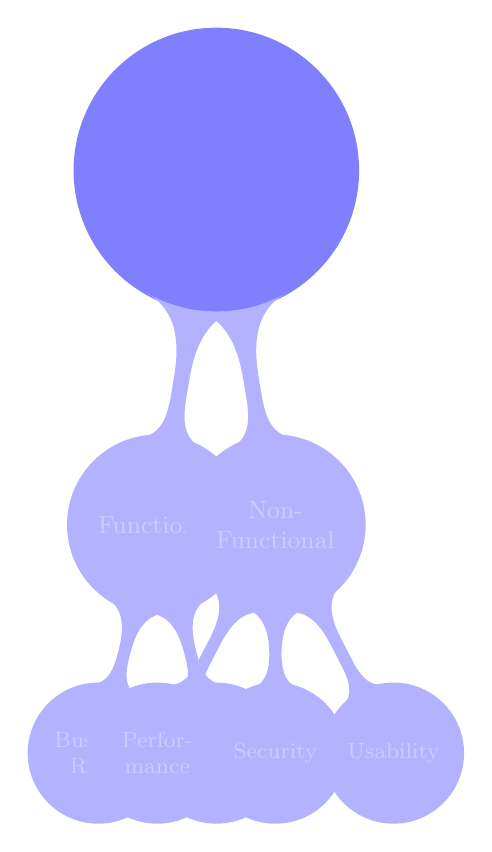
\begin{tikzpicture}[
    mindmap,
    concept color=blue!30,
    every node/.style={concept, execute at begin node=\hskip0pt},
    root concept/.append style={concept, color=blue!50, minimum size=3cm, font=\bfseries},
    level 1 concept/.append style={level distance=4.5cm, sibling angle=90, color=blue!20}
]
    \node [root concept] {Requirements}
        child { node {Functional} 
            child { node {Business\\Rules} }
            child { node {User\\Actions} }
        }
        child { node {Non-Functional} 
            child { node {Performance} }
            child { node {Security} }
            child { node {Usability} }
        };
\end{tikzpicture}
\captionof{figure}{Requirement Types}
\end{center}
\end{solutionbox}

\begin{mnemonicbox}
\mnemonic{Functional = What, Non-Functional = How}
\end{mnemonicbox}

\questionmarks{3(a OR)}{3}{Describe skill to manage software projects}

\begin{solutionbox}
Project management requires diverse skill set for successful software delivery.

\textbf{Essential Skills:}
\begin{center}
\captionof{table}{PM Skills}
\begin{tabulary}{\linewidth}{|L|L|L|}
\hline
\textbf{Skill Category} & \textbf{Description} & \textbf{Application} \\ \hline
\textbf{Technical} & Understanding technology & Architecture decisions \\ \hline
\textbf{Leadership} & Team motivation & Conflict resolution \\ \hline
\textbf{Communication} & Stakeholder interaction & Status reporting \\ \hline
\end{tabulary}
\end{center}
\end{solutionbox}

\begin{mnemonicbox}
\mnemonic{Technical Leadership Communication}
\end{mnemonicbox}

\questionmarks{3(b OR)}{4}{Briefly give the Responsibility of software project Manager.}

\begin{solutionbox}
Software Project Manager oversees entire project lifecycle and ensures successful delivery.

\textbf{Key Responsibilities:}
\begin{center}
\captionof{table}{PM Responsibilities}
\begin{tabulary}{\linewidth}{|L|L|L|}
\hline
\textbf{Area} & \textbf{Responsibility} & \textbf{Activities} \\ \hline
\textbf{Planning} & Project roadmap & Schedule, budget, resource allocation \\ \hline
\textbf{Execution} & Team coordination & Task assignment, progress monitoring \\ \hline
\textbf{Quality} & Standard compliance & Code reviews, testing oversight \\ \hline
\textbf{Communication} & Stakeholder updates & Status reports, risk communication \\ \hline
\end{tabulary}
\end{center}

\textbf{Additional Duties:}
\begin{itemize}
    \item \keyword{Risk Management}: Identify and mitigate project risks
    \item \keyword{Team Development}: Mentor team members and resolve conflicts
\end{itemize}

\begin{center}
\begin{tikzpicture}[node distance=1.5cm, auto, every node/.style={gtu block, align=center, font=\small}]
    \node (PM) [fill=yellow!20] {Project Manager};
    \node [above=of PM] (Plan) {Planning};
    \node [right=of PM] (Exec) {Execution};
    \node [below=of PM] (Qual) {Quality};
    \node [left=of PM] (Comm) {Communication};

    \path [gtu arrow] (PM) -- (Plan);
    \path [gtu arrow] (PM) -- (Exec);
    \path [gtu arrow] (PM) -- (Qual);
    \path [gtu arrow] (PM) -- (Comm);
\end{tikzpicture}
\captionof{figure}{PM Functions}
\end{center}
\end{solutionbox}

\begin{mnemonicbox}
\mnemonic{Plan Execute Quality Communicate Risk Team}
\end{mnemonicbox}

\questionmarks{3(c OR)}{7}{Compare PERT chart – Gantt chart side by side.}

\begin{solutionbox}
Both charts are project management tools but serve different purposes and have distinct characteristics.

\textbf{Detailed Comparison:}
\begin{center}
\captionof{table}{PERT vs Gantt}
\begin{tabulary}{\linewidth}{|L|L|L|}
\hline
\textbf{Aspect} & \textbf{PERT Chart} & \textbf{Gantt Chart} \\ \hline
\textbf{Purpose} & Show task dependencies & Show project timeline \\ \hline
\textbf{Structure} & Network diagram & Bar chart \\ \hline
\textbf{Focus} & Critical path analysis & Schedule visualization \\ \hline
\textbf{Time Display} & Estimated durations & Actual dates \\ \hline
\textbf{Dependencies} & Explicit arrows & Implicit connections \\ \hline
\textbf{Best For} & Complex projects & Simple scheduling \\ \hline
\end{tabulary}
\end{center}

\textbf{Visual Representation:}
\begin{center}
\begin{tikzpicture}[node distance=1.5cm, auto, every node/.style={circle, draw, font=\small}]
    \node (A) {A};
    \node (B) [below=of A] {B};
    \node (C) [right=of A] {C};
    \node (D) [right=of C] {D};
    
    \path [gtu arrow] (A) -- (C);
    \path [gtu arrow] (B) -- (C);
    \path [gtu arrow] (C) -- (D);
\end{tikzpicture}
\captionof{figure}{PERT Chart Concept}
\end{center}

\begin{center}
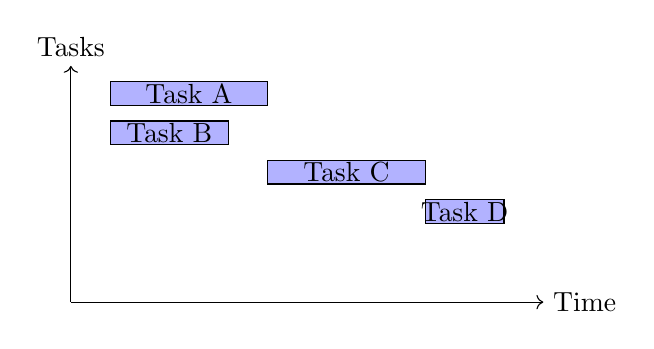
\begin{tikzpicture}
    % Gantt chart approximate
    \draw[->] (0,0) -- (6,0) node[right] {Time};
    \draw[->] (0,0) -- (0,3) node[above] {Tasks};
    
    \draw[fill=blue!30] (0.5, 2.5) rectangle (2.5, 2.8) node[midway] {Task A};
    \draw[fill=blue!30] (0.5, 2.0) rectangle (2.0, 2.3) node[midway] {Task B};
    \draw[fill=blue!30] (2.5, 1.5) rectangle (4.5, 1.8) node[midway] {Task C};
    \draw[fill=blue!30] (4.5, 1.0) rectangle (5.5, 1.3) node[midway] {Task D};
\end{tikzpicture}
\captionof{figure}{Gantt Chart Concept}
\end{center}

\textbf{When to Use:}
\begin{center}
\captionof{table}{Usage Guide}
\begin{tabulary}{\linewidth}{|L|L|L|}
\hline
\textbf{Scenario} & \textbf{PERT} & \textbf{Gantt} \\ \hline
\textbf{Project Type} & Research \& Development & Construction, Software \\ \hline
\textbf{Uncertainty} & High uncertainty & Well-defined tasks \\ \hline
\textbf{Audience} & Technical team & Management, Clients \\ \hline
\end{tabulary}
\end{center}

\textbf{Advantages Comparison:}
\begin{itemize}
    \item \textbf{PERT}: Critical path, Flexible timing, Risk analysis
    \item \textbf{Gantt}: Easy to understand, Progress tracking, Resource allocation
\end{itemize}
\end{solutionbox}

\begin{mnemonicbox}
\mnemonic{PERT = Path, Gantt = Bars}
\end{mnemonicbox}

\questionmarks{4(a)}{3}{Give steps of Project Monitoring and control process}

\begin{solutionbox}
Project monitoring ensures project stays on track through systematic observation and corrective actions.

\textbf{Monitoring Steps:}
\begin{center}
\captionof{table}{Process Steps}
\begin{tabulary}{\linewidth}{|L|L|L|}
\hline
\textbf{Step} & \textbf{Activity} & \textbf{Purpose} \\ \hline
\textbf{Track Progress} & Measure actual vs planned & Identify deviations \\ \hline
\textbf{Assess Quality} & Review deliverables & Ensure standards \\ \hline
\textbf{Take Action} & Implement corrections & Maintain alignment \\ \hline
\end{tabulary}
\end{center}
\end{solutionbox}

\begin{mnemonicbox}
\mnemonic{Track Assess Take}
\end{mnemonicbox}

\questionmarks{4(b)}{4}{Discuss i)Risk Assessment ii)Risk Mitigation}

\begin{solutionbox}
\textbf{(i) Risk Assessment:}
Process of identifying and evaluating potential project risks.
\begin{center}
\captionof{table}{Assessment Components}
\begin{tabulary}{\linewidth}{|L|L|L|}
\hline
\textbf{Assessment Type} & \textbf{Method} & \textbf{Output} \\ \hline
\textbf{Risk Identification} & Brainstorming, checklists & Risk list \\ \hline
\textbf{Risk Analysis} & Probability $\times$ Impact & Risk priority \\ \hline
\textbf{Risk Evaluation} & Risk matrix & Action priorities \\ \hline
\end{tabulary}
\end{center}

\textbf{(ii) Risk Mitigation:}
Strategies to reduce risk impact and probability.
\begin{center}
\captionof{table}{Mitigation Strategies}
\begin{tabulary}{\linewidth}{|L|L|L|}
\hline
\textbf{Strategy} & \textbf{Description} & \textbf{Example} \\ \hline
\textbf{Avoidance} & Eliminate risk source & Change technology \\ \hline
\textbf{Reduction} & Minimize impact & Add testing \\ \hline
\textbf{Transfer} & Shift risk to others & Insurance, outsourcing \\ \hline
\textbf{Acceptance} & Live with risk & Contingency planning \\ \hline
\end{tabulary}
\end{center}
\end{solutionbox}

\begin{mnemonicbox}
\mnemonic{Avoid Reduce Transfer Accept}
\end{mnemonicbox}

\questionmarks{4(c)}{7}{Define project risk and how Manage Risk Management it.}

\begin{solutionbox}
Project Risk is an uncertain event that, if occurs, has positive or negative effect on project objectives.

\textbf{Risk Characteristics:}
\begin{center}
\captionof{table}{Characteristics}
\begin{tabulary}{\linewidth}{|L|L|L|}
\hline
\textbf{Characteristic} & \textbf{Description} & \textbf{Example} \\ \hline
\textbf{Uncertainty} & May or may not occur & Technology failure \\ \hline
\textbf{Impact} & Affects project parameters & Cost, schedule, quality \\ \hline
\textbf{Probability} & Likelihood of occurrence & 30\% chance of delay \\ \hline
\end{tabulary}
\end{center}

\textbf{Risk Management Process:}
\begin{center}
\begin{tikzpicture}[node distance=1.5cm, auto, every node/.style={gtu state, align=center, font=\footnotesize}]
    \node (Ident) {Identify};
    \node [right=of Ident] (Assess) {Assess};
    \node [right=of Assess] (Prior) {Prioritize};
    \node [below=of Prior] (Resp) {Response};
    \node [left=of Resp] (Mon) {Monitor};
    \node [left=of Mon] (Cont) {Control};

    \path [gtu arrow] (Ident) -- (Assess);
    \path [gtu arrow] (Assess) -- (Prior);
    \path [gtu arrow] (Prior) -- (Resp);
    \path [gtu arrow] (Resp) -- (Mon);
    \path [gtu arrow] (Mon) -- (Cont);
    \path [gtu arrow] (Cont) -- (Ident);
\end{tikzpicture}
\captionof{figure}{Management Loop}
\end{center}

\textbf{Risk Management Steps:}
\begin{center}
\captionof{table}{Process Details}
\begin{tabulary}{\linewidth}{|L|L|L|L|}
\hline
\textbf{Step} & \textbf{Activities} & \textbf{Tools} & \textbf{Output} \\ \hline
\textbf{Identification} & Brainstorming & Checklists, SWOT & Risk register \\ \hline
\textbf{Assessment} & Prob/Impact analysis & Risk matrix & Risk ratings \\ \hline
\textbf{Response} & Develop strategies & Response templates & Action plans \\ \hline
\textbf{Monitoring} & Track indicators & Dashboards & Status reports \\ \hline
\end{tabulary}
\end{center}

\textbf{Risk Response Strategies:}
\begin{itemize}
    \item \keyword{Negative Risks}: Avoid, Transfer, Mitigate, Accept
    \item \keyword{Positive Risks}: Exploit, Share, Enhance, Accept
\end{itemize}
\end{solutionbox}

\begin{mnemonicbox}
\mnemonic{Identify Assess Respond Monitor + Avoid Transfer Mitigate Accept}
\end{mnemonicbox}

\questionmarks{4(a OR)}{3}{Describe Software design process and explain Design methodologies.}

\begin{solutionbox}
Software design transforms requirements into blueprint for implementation through systematic approach.

\textbf{Design Process:}
\begin{center}
\captionof{table}{Process Structure}
\begin{tabulary}{\linewidth}{|L|L|L|}
\hline
\textbf{Phase} & \textbf{Activity} & \textbf{Output} \\ \hline
\textbf{Analysis} & Understand requirements & Problem definition \\ \hline
\textbf{Architecture} & High-level structure & System architecture \\ \hline
\textbf{Detailed Design} & Component specification & Design documents \\ \hline
\end{tabulary}
\end{center}
\end{solutionbox}

\begin{mnemonicbox}
\mnemonic{Analysis Architecture Detail}
\end{mnemonicbox}

\questionmarks{4(b OR)}{4}{Compare Cohesion and Coupling side by side.}

\begin{solutionbox}
Both concepts measure module design quality but focus on different aspects.

\textbf{Comprehensive Comparison:}
\begin{center}
\captionof{table}{Cohesion vs Coupling}
\begin{tabulary}{\linewidth}{|L|L|L|}
\hline
\textbf{Aspect} & \textbf{Cohesion} & \textbf{Coupling} \\ \hline
\textbf{Definition} & Degree of relatedness within module & Degree of interdependence between modules \\ \hline
\textbf{Goal} & High cohesion desired & Low coupling desired \\ \hline
\textbf{Focus} & Internal module structure & Inter-module relationships \\ \hline
\textbf{Quality} & Stronger = Better & Weaker = Better \\ \hline
\end{tabulary}
\end{center}

\textbf{Types Comparison (Best to Worst):}
\begin{itemize}
    \item \keyword{Cohesion}: Functional, Sequential, Communicational, Procedural, Temporal, Logical, Coincidental
    \item \keyword{Coupling}: Data, Stamp, Control, External, Common, Content
\end{itemize}

\textbf{Impact on Design:}
High cohesion and low coupling leads to better maintainability, reusability, and testing.
\end{solutionbox}

\begin{mnemonicbox}
\mnemonic{Cohesion = Inside Strong, Coupling = Between Weak}
\end{mnemonicbox}

\questionmarks{4(c OR)}{7}{Sketch Data Flow Diagram with levels and explain.}

\begin{solutionbox}
Data Flow Diagram (DFD) shows how data moves through system using graphical notation with multiple levels of detail.

\textbf{DFD Levels:}
\begin{center}
\begin{tikzpicture}[node distance=1.5cm, auto, every node/.style={gtu block, align=center, font=\footnotesize}]
    \node (L0) {Level 0\\Context Diagram};
    \node [right=of L0] (L1) {Level 1\\Major Processes};
    \node [right=of L1] (L2) {Level 2\\Sub-processes};
    \node [right=of L2] (L3) {Level 3\\Detailed};

    \path [gtu arrow] (L0) -- (L1);
    \path [gtu arrow] (L1) -- (L2);
    \path [gtu arrow] (L2) -- (L3);
\end{tikzpicture}
\captionof{figure}{DFD Levels}
\end{center}

\textbf{Level Descriptions:}
\begin{center}
\captionof{table}{Level Details}
\begin{tabulary}{\linewidth}{|L|L|L|L|}
\hline
\textbf{Level} & \textbf{Scope} & \textbf{Purpose} & \textbf{Detail} \\ \hline
\textbf{Level 0} & Entire system & System boundary & Single process \\ \hline
\textbf{Level 1} & Major functions & High-level processes & 5-7 processes \\ \hline
\textbf{Level 2} & Sub-functions & Process breakdown & Detailed view \\ \hline
\textbf{Level 3+} & Fine details & Implementation level & Very specific \\ \hline
\end{tabulary}
\end{center}

\textbf{Example - Level 1 DFD:}
\begin{center}
\begin{tikzpicture}[node distance=1.5cm, auto, every node/.style={font=\footnotesize}]
    \node (Stu) [draw, rectangle] {Student};
    \node (P1) [draw, circle, right=of Stu] {1.0 Register};
    \node (DB) [draw, cylinder, shape border rotate=90, aspect=0.25, right=of P1] {Student DB};
    \node (P2) [draw, circle, right=of DB] {2.0 Report};
    \node (Adm) [draw, rectangle, right=of P2] {Admin};

    \path [gtu arrow] (Stu) -- (P1);
    \path [gtu arrow] (P1) -- (DB);
    \path [gtu arrow] (DB) -- (P2);
    \path [gtu arrow] (P2) -- (Adm);
\end{tikzpicture}
\captionof{figure}{Level 1 Example}
\end{center}

\textbf{Benefits:}
Abstraction, Decomposition, Verification.
\end{solutionbox}

\begin{mnemonicbox}
\mnemonic{Context Major Sub Fine + Process Entity Store Flow}
\end{mnemonicbox}

\questionmarks{5(a)}{3}{Give Characteristics of good UI.}

\begin{solutionbox}
Good User Interface design ensures effective user interaction with software system.

\textbf{UI Characteristics:}
\begin{center}
\captionof{table}{Key Features}
\begin{tabulary}{\linewidth}{|L|L|L|}
\hline
\textbf{Characteristic} & \textbf{Description} & \textbf{Benefit} \\ \hline
\textbf{Simple} & Easy to understand & Reduced learning curve \\ \hline
\textbf{Consistent} & Uniform behavior & Predictable interaction \\ \hline
\textbf{Responsive} & Quick feedback & User satisfaction \\ \hline
\end{tabulary}
\end{center}
\end{solutionbox}

\begin{mnemonicbox}
\mnemonic{Simple Consistent Responsive}
\end{mnemonicbox}

\questionmarks{5(b)}{4}{Briefly explain Unit testing}

\begin{solutionbox}
Unit Testing verifies individual software components in isolation to ensure correct functionality.

\textbf{Unit Testing Overview:}
\begin{center}
\captionof{table}{Testing Scope}
\begin{tabulary}{\linewidth}{|L|L|L|}
\hline
\textbf{Aspect} & \textbf{Description} & \textbf{Purpose} \\ \hline
\textbf{Scope} & Individual modules & Component verification \\ \hline
\textbf{Isolation} & Test in isolation & Independent validation \\ \hline
\textbf{Automation} & Automated execution & Efficient testing \\ \hline
\textbf{Early Detection} & Find bugs early & Cost-effective \\ \hline
\end{tabulary}
\end{center}

\begin{center}
\begin{tikzpicture}[node distance=1.2cm, auto, every node/.style={gtu block, align=center, font=\small}]
    \node (Test) {Write Test Cases};
    \node [right=of Test] (Exec) {Execute Tests};
    \node [right=of Exec] (Res) {Analyze Results};
    \node [right=of Res] (Fix) {Fix Defects};
    
    \path [gtu arrow] (Test) -- (Exec);
    \path [gtu arrow] (Exec) -- (Res);
    \path [gtu arrow] (Res) -- (Fix);
    \path [gtu arrow] (Fix) to [bend left] (Exec);
\end{tikzpicture}
\captionof{figure}{Unit Testing Cycle}
\end{center}

\textbf{Benefits:}
Early bug detection, Code quality improvement, Regression testing.
\end{solutionbox}

\begin{mnemonicbox}
\mnemonic{Scope Isolation Automation Early}
\end{mnemonicbox}

\questionmarks{5(c)}{7}{Draw activity diagrams of the train reservation system, explain each step.}

\begin{solutionbox}
Activity Diagram shows workflow of train reservation system from user request to ticket confirmation.

\begin{center}
\begin{tikzpicture}[node distance=1.5cm, auto, every node/.style={gtu block, align=center, font=\footnotesize}]
    \node (Start) [gtu start] {Start};
    \node (Login) [below=0.8cm of Start] {User Login};
    \node (Cred) [gtu decision, below=0.8cm of Login] {Valid?};
    \node (Search) [below=0.8cm of Cred] {Search Trains};
    \node (Select) [below=0.8cm of Search] {Select Train};
    \node (Details) [right=of Search] {Enter Details};
    \node (Review) [right=of Details] {Review Booking};
    \node (Pay) [below=0.8cm of Review] {Process Payment};
    \node (Success) [gtu decision, below=0.8cm of Pay] {Success?};
    \node (Gen) [below=0.8cm of Success] {Generate Ticket};
    \node (End) [gtu stop, below=0.8cm of Gen] {End};

    \path [gtu arrow] (Start) -- (Login);
    \path [gtu arrow] (Login) -- (Cred);
    \path [gtu arrow] (Cred) -- node[right] {Yes} (Search);
    \path [gtu arrow] (Cred) to [bend right] node[left] {No} (Login);
    \path [gtu arrow] (Search) -- (Select);
    \path [gtu arrow] (Select) -| (Details);
    \path [gtu arrow] (Details) -- (Review);
    \path [gtu arrow] (Review) -- (Pay);
    \path [gtu arrow] (Pay) -- (Success);
    \path [gtu arrow] (Success) -- node[right] {Yes} (Gen);
    \path [gtu arrow] (Success) to [bend right] node[left] {No} (Pay);
    \path [gtu arrow] (Gen) -- (End);
\end{tikzpicture}
\captionof{figure}{Train Reservation Activity}
\end{center}

\textbf{Step Explanation:}
\begin{itemize}
    \item \textbf{Login}: User authentication.
    \item \textbf{Search}: Find trains for route/date.
    \item \textbf{Selection}: Choose train and seats.
    \item \textbf{Details}: Enter passenger info.
    \item \textbf{Payment}: Process transaction.
    \item \textbf{Ticket}: Generate and send confirmation.
\end{itemize}
\end{solutionbox}

\begin{mnemonicbox}
\mnemonic{Login Search Select Choose Enter Review Pay Generate Send}
\end{mnemonicbox}

\questionmarks{5(a OR)}{3}{Compare Verification, Validation side by side.}

\begin{solutionbox}
Both are quality assurance activities but focus on different aspects of correctness.

\textbf{Verification vs Validation:}
\begin{center}
\captionof{table}{Comparison}
\begin{tabulary}{\linewidth}{|L|L|L|}
\hline
\textbf{Aspect} & \textbf{Verification} & \textbf{Validation} \\ \hline
\textbf{Question} & "Are we building right?" & "Are we building right thing?" \\ \hline
\textbf{Focus} & Process correctness & Product correctness \\ \hline
\textbf{Method} & Reviews, inspections & Testing, user feedback \\ \hline
\end{tabulary}
\end{center}
\end{solutionbox}

\begin{mnemonicbox}
\mnemonic{Verification = Right Process, Validation = Right Product}
\end{mnemonicbox}

\questionmarks{5(b OR)}{4}{Define Testing describe any two testing type.}

\begin{solutionbox}
Testing is process of evaluating software to detect errors and ensure it meets requirements.

\textbf{Two Testing Types:}
\begin{center}
\captionof{table}{Black Box vs White Box}
\begin{tabulary}{\linewidth}{|L|L|L|}
\hline
\textbf{Aspect} & \textbf{Black Box} & \textbf{White Box} \\ \hline
\textbf{Approach} & Unknown internal structure & Known code structure \\ \hline
\textbf{Focus} & Functional requirements & Internal logic \\ \hline
\textbf{Tester} & User acceptance & Developer unit testing \\ \hline
\end{tabulary}
\end{center}
\end{solutionbox}

\begin{mnemonicbox}
\mnemonic{Black = External, White = Internal}
\end{mnemonicbox}

\questionmarks{5(c OR)}{7}{Describe each Coding standards and guidelines.}

\begin{solutionbox}
Coding Standards are rules for writing consistent, maintainable code.

\textbf{Major Categories:}
\begin{enumerate}
    \item \textbf{Naming Conventions}: camelCase for variables, PascalCase for classes.
    \item \textbf{Code Structure}: Consistent indentation, line length limits.
    \item \textbf{Organization}: Single responsibility, small functions.
    \item \textbf{Documentation}: Header comments, meaningful inline comments.
    \item \textbf{Error Handling}: Graceful exception handling, logging.
    \item \textbf{Performance}: Avoid memory leaks, efficient algorithms.
\end{enumerate}

\begin{center}
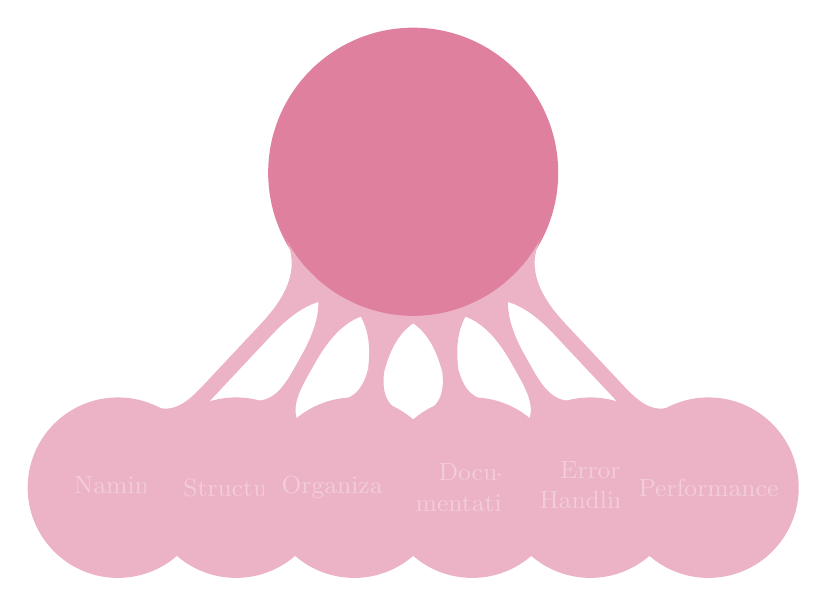
\begin{tikzpicture}[
    mindmap,
    concept color=purple!30,
    every node/.style={concept, execute at begin node=\hskip0pt},
    root concept/.append style={concept, color=purple!50, minimum size=3cm, font=\bfseries},
    level 1 concept/.append style={level distance=4cm, sibling angle=60, color=purple!20}
]
    \node [root concept] {Coding\\Standards}
        child { node {Naming} }
        child { node {Structure} }
        child { node {Organization} }
        child { node {Documentation} }
        child { node {Error\\Handling} }
        child { node {Performance} };
\end{tikzpicture}
\captionof{figure}{Standard Categories}
\end{center}

\textbf{Benefits:}
Improved readability, consistency, maintainability, and quality.
\end{solutionbox}

\begin{mnemonicbox}
\mnemonic{Name Structure Organize Document Handle Perform Review}
\end{mnemonicbox}

\end{document}
